\section{Frozen protocols and additional results}
\label{app:protocols}

\subsection{Matrix-Game commitment and rollback gates}

\paragraph{Commitment calibration.}
The calibration set contains official universal images 0000--0007 and both
mouse-left$\leftrightarrow$mouse-right directions. For each of the 16
direction-scene pairs, the runner generates the \new{} and \old{} oracles and
the two interior switch points. Prefix, prompt-free image conditioning, initial
current-block latent, future noise tensors, weights, sampler, precision, cache
history, and non-action conditioning are exact across branches. The intended
action tensor is the only difference. All 16 pairs pass oracle distinction,
tracking support, monotonicity, boundedness, temporal quality, and latent
coupling.

\begin{table}[h]
  \centering
  \caption{Frozen Matrix-Game commitment curve. Values are medians over 16
  valid direction-scene pairs.}
  \small
  \begin{tabular}{lrrrr}
    \toprule
    OLD-action NFEs $s$ & 0 & 1 & 2 & 3 \\
    \midrule
    Normalized response $R(s)$ & 1.0000 & 0.9971 & 0.2182 & 0.0000 \\
    \bottomrule
  \end{tabular}
\end{table}

\paragraph{Gate 1 rollback.}
The 16 calibration pairs compare \direct{}, exact rollback of the minimal
suffix, and full restart with identical stochastic inputs. Minimal rollback is within 0.10 of
restart on 16/16 pairs and improves over direct binding on 16/16. Median
responses are 0.2182/0.9971/1.0000 for direct/minimal/restart, and minimal
rollback has median future-SSIM 0.9026.

\subsection{Exact Matrix-Game runtime state}

Matrix-Game routes causal self-attention KV insertion through a single cache
operation immediately before attention reads. Runtime tracing shows that every
current-block visual and active action KV position is overwritten before use
at \nfe{}2. Historical prefix KV and cross-attention KV therefore remain live
by reference rather than being copied.

\begin{table}[h]
  \centering
  \caption{Exact checkpoint storage. The final implementation removes
  overwritten state, not numerical information required by replay.}
  \small
  \begin{tabular}{lr}
    \toprule
    Payload & Bytes \\
    \midrule
    Entering-\nfe{}2 BF16 latent $[1,16,3,44,80]$ & 337,920 \\
    Defensive visual/mouse/keyboard cache indices & 1,440 \\
    \textbf{Implemented exact checkpoint} & \textbf{339,360} \\
    Mathematical minimum (latent plus step) & 337,928 \\
    Initial exact implementation & 649,330,080 \\
    \bottomrule
  \end{tabular}
\end{table}

The final checkpoint is $1{,}913\times$ smaller than the initial
implementation and 1,432 bytes (0.424\%) above the measured logical minimum.
Median save/restore times are 1.456/0.878\,ms. The full live per-fork cache
allocation is 1,670,124,960 bytes but is not duplicated by \method{}.

\subsection{Asynchronous serving details}

The primary serving set uses official images 0008--0015 with four deterministic
prefix-noise variants each. All 32 contexts and both yaw directions are
retained. Each direction receives 16 deterministic stratified-uniform arrival
times over the wall-clock support of the three old-action evaluations, using
one frozen seed family. The resulting classes contain 348 \nfe{}1 arrivals,
338 \nfe{}2 arrivals, and 338 \nfe{}3 arrivals.

The serving hierarchy has eight independent base images, four deterministic
variants per base, two directions per variant, and 16 arrivals per direction.
Late arrivals have \texttt{inflight\_nfe $\geq$ 2}, retaining 676 of 1,024
rows. Inference averages late rows within direction and the eight derived
variant/direction cells within each base, then treats the eight base images as
clusters. The late-arrival \method{}-minus-\direct{} response effect has mean
0.909136, median 0.930385, and base-cluster bootstrap 95\% CI
$[0.859769,0.954093]$; all 8/8 base effects are positive (exact one-/two-sided
Wilcoxon $p=0.00390625/0.0078125$). The fixed per-direction
\texttt{lateact-direct\_late} branch contrast is a distinct descriptive
$n=64$ estimand (mean 0.815919), not the mean over the 676 asynchronous late
rows.

Full-restart-minus-\method{} latency saving across the eight base clusters has
mean 0.311789\,s, median 0.313654\,s, and 95\% CI
$[0.305519,0.317523]$\,s; 8/8 are positive with the same exact Wilcoxon
values. The frozen mean saving fraction is 11.93\%. Every late case is within
0.10 normalized response of restart and uses fewer redone evaluations. All
348 early cases use exactly zero rollback.

\subsection{Mouse-yaw trajectory-quality tail}
\label{app:quality}

The 64 scene-variant/direction comparisons are descriptive quality units. The
future-SSIM distribution has mean 0.915660, median 0.922305, p05 0.839679, and
minimum 0.718375. Counts at least 0.90/0.85/0.80 are 49/64, 60/64, and 63/64;
equivalently 15/64, 4/64, and 1/64 fall below those values. Sub-0.90 values
occur in four base images; base 0013 contains 6/8 and the sole value below
0.80. Thus mouse-yaw trajectory quality is broadly stable but not uniform.
The frozen SSIM $\geq0.90$ gate is a median-level safeguard, not a per-example
threshold, and no tail cutoff is introduced retrospectively.

Temporal difference (\method{} minus \new{}) has median +0.001691 and range
$[-0.007878,0.018057]$; temporal and finite/nonconstant decode safeguards pass
64/64.

\begin{figure}[h]
  \centering
  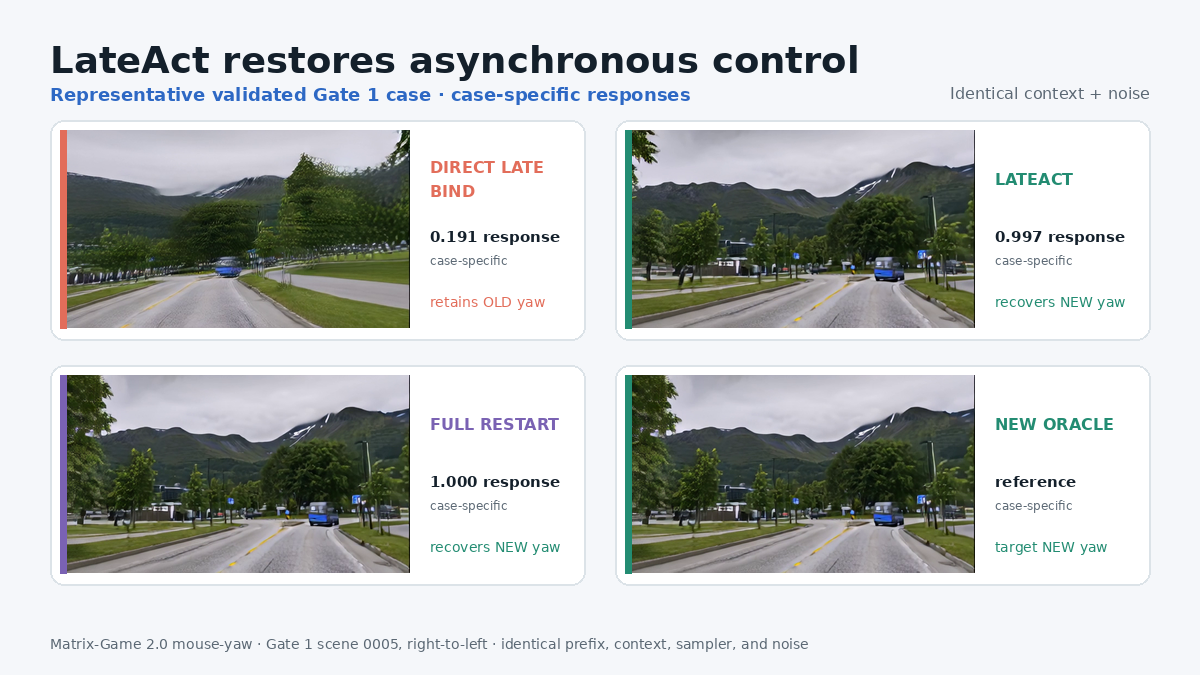
\includegraphics[width=0.72\linewidth]{figures/matrix_qualitative.png}
  \caption{Representative coupled Matrix-Game mouse-yaw branch. Direct late
  binding retains the old yaw (response 0.191), while \method{} (0.997) tracks
  full restart (1.000) in normalized action response. This favorable example
  is not the quality-tail evidence and was not used to set thresholds.}
  \label{fig:qualitative}
\end{figure}

\subsection{Gate rationale}

The frozen numerical cutoffs are safeguards against specific invalidating
conditions, not uniquely privileged constants. The 8-pixel oracle gap demands
minimum absolute action separation; the $10\times$ same-action floor demands
separation well above repeatability noise; and at least 20 motion inliers
protects the affine estimate from sparse tracking. A 0.10 normalized-response
gap is the operational near-restart tolerance. Median future-SSIM $\geq0.90$
protects trajectory fidelity without requiring every example to exceed 0.90.
Finally, a median adjacent response drop of at least 0.15 distinguishes a
materially steep transition at the available NFE granularity from a flat or
noisy curve.

\subsection{minWM frozen chronology}
\label{app:minwm}

\paragraph{Original lateral control.}
The original minWM protocol fixes prompts 0--7, seeds 41000--41007, actions
\texttt{a*3}/\texttt{d*3}, both directions, and $s=0,\ldots,4$. The
same-action decoded floor is 0.0776 pixels. Oracle affine gaps have median
6.851 pixels and range 1.169--12.767; only three scenes in both directions
exceed the fixed 8-pixel threshold, yielding 6/16 valid pairs. The
formal replication verdict is failure even though all 16 raw curves are
monotone and bounded and show a median first drop of 0.9566.

\paragraph{Frozen yaw confirmation.}
After the lateral identifiability failure was established, exactly one bounded
follow-up protocol was frozen at commit \texttt{f1e2bbc} before confirmatory
outputs were generated. It fixes fresh consecutive official prompts 8--15,
seeds 41008--41015, native \texttt{j*3}/\texttt{l*3} yaw, both switch
directions, the unchanged evaluator, thresholds, and success gate. Prompt
screening/replacement, alternative evaluators or actions, and rollback are
prohibited. This is a pre-specified frozen follow-up after a failed
identifiability audit; the adaptive chronology is explicit, and the protocol
was fixed before confirmatory execution.

\begin{table}[h]
  \centering
  \caption{Per-scene minWM yaw oracle separation. The signed value reverses
  between directions; absolute gap and inlier support are shared.}
  \small
  \begin{tabular}{lrrc}
    \toprule
    Scene & Absolute gap (px) & Median oracle inliers & Valid directions \\
    \midrule
    08 & 35.359 & 177.0 & 2/2 \\
    09 & 14.002 & 833.5 & 2/2 \\
    10 & 13.982 & 690.5 & 2/2 \\
    11 & 35.345 & 469.5 & 2/2 \\
    12 & 10.238 & 298.5 & 2/2 \\
    13 & 19.007 & 246.0 & 2/2 \\
    14 & 19.035 & 631.5 & 2/2 \\
    15 & 45.441 & 399.5 & 2/2 \\
    \bottomrule
  \end{tabular}
\end{table}

The same-action control ranges are 0.3892 and 0.6580 pixels; the latter is the
frozen repeatability floor, giving a $10\times$ requirement of 6.5801 pixels.
All 16 pairs exceed both this value and 8 pixels. Affine/LK signs agree 16/16,
all median inlier counts exceed 20, all videos are valid, and all 16 curves are
monotone and bounded. Exact branch-noise hashes, historical/cross-sampled
state, and four-evaluation counts pass on all eight scenes. Same-action latent
hashes are exact on both control prompts.

\subsection{Keyboard chronology}
\label{app:keyboard}

The initial eight-context keyboard transfer used the mouse-yaw score and
reported asymmetric response. The subsequent diagnostic froze an
action-appropriate signed lateral translation evaluator before generating
broad results. On 10 calibration contexts and 20 directions, all directions
are valid; median response is 0.9957 at $s=1$ and 0.1240 at $s=2$, placing the
latest safe state after \nfe{}1, exactly as for mouse-yaw.

The confirmation uses 24 disjoint stochastic contexts, 48 directions, and 16
arrivals per direction. Mouse-boundary and action-specific policies are the
same algorithm and are bit-exact on 768/768 records. Median response is 1.0188;
all 512 late arrivals are within 0.10 of restart and save 0.3105\,s median.
Nevertheless, median future-SSIM to \new{} is 0.6726 (range
0.5989--0.9139), failing the frozen median-level 0.90 threshold. Temporal consistency passes
48/48. The videos are coherent but follow a different exact trajectory.

\section{Reproducibility and audit details}
\label{app:repro}
\label{app:audits}
\label{app:compute}

No model is trained or fine-tuned. The experiments use released Matrix-Game
2.0 and minWM Wan2.1 Action2V checkpoints, BF16 inference, deterministic
materialized future noise, and frozen YAML protocols. Runners, analyzers,
protocol validators, configs, and lightweight reports are retained for an
anonymous release; large checkpoints and generated videos are excluded.

For each scientific branch, the runner records hashes of action tensors,
initial and re-noising tensors, prefix latents, cache indices, sampled
historical cache bytes, cross-attention state, and output latents. Analyzer
guards reject prompt substitution, action mismatch, threshold drift, output
overwrite, insufficient oracle separation, evaluator-sign disagreement,
non-finite videos, and failed same-action equality.

Matrix-Game generation uses two NVIDIA RTX 3090 GPUs. The primary serving
runner measures 955.60 synchronized GPU-seconds across 64 scene-directions
(6.21\,s generation and 8.72\,s decode per bundle). minWM uses one RTX 3090;
74 confirmatory branches average 6.156\,s generation and 7.417\,s decode
(1,004.42 timed GPU-seconds total), with 19,340,754,432 peak allocated bytes.

\section{Existing assets and broader impact}
\label{app:impact}

The work evaluates released Matrix-Game 2.0 and minWM implementations and
checkpoints and cites their corresponding papers. The Matrix-Game 2.0 source
release identifies an MIT license; minWM is released under Apache-2.0. Model
checkpoints and official evaluation assets are used under their respective
upstream terms and are not redistributed in the submission.

Commitment-aware rollback can reduce wasted inference and make interactive
world-model feedback more responsive, which may benefit embodied-agent
simulation and human-in-the-loop control. The same capability can also make
synthetic environments more persuasive despite incorrect dynamics. A
particularly relevant failure mode is false confidence: recovering an
action-direction metric does not guarantee recovery of the exact intended
trajectory, as demonstrated by the keyboard SSIM failure. These systems should
therefore not control safety-critical physical hardware solely from the
evaluated pixel or motion metrics. Deployment would require task-level state
validation, uncertainty monitoring, safe fallback behavior, and evaluation on
the target embodiment.
